% Auto-generated by scripts/inspect_geometry_v2.jl
\documentclass{article}
\usepackage[margin=1.5cm]{geometry}
\usepackage{tikz}
\usepackage{xcolor}
\usepackage{graphicx}
\pagestyle{empty}
\begin{document}
\begin{figure}[p]
\centering
\resizebox{0.45\linewidth}{!}{%
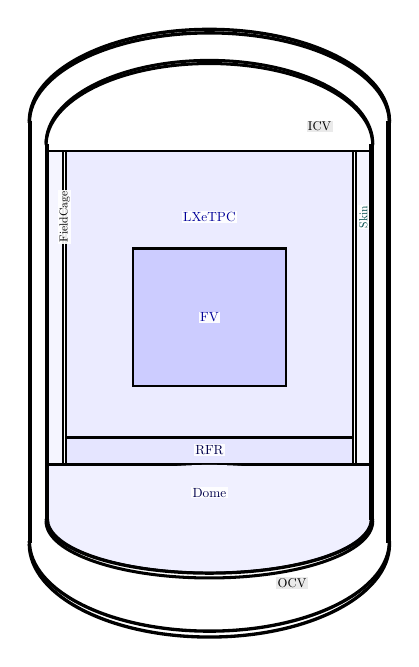
\begin{tikzpicture}[x=0.025cm,y=0.025cm]
\path[fill=blue!8, draw=none] (-72.800, 0.000) rectangle (72.800, 145.600);
\draw[black, line width=0.8pt] (-72.800, 0.000) rectangle (72.800, 145.600);
\path[fill=blue!20, draw=none] (-39.000, 26.000) rectangle (39.000, 96.000);
\draw[black, line width=0.8pt] (-39.000, 26.000) rectangle (39.000, 96.000);
\draw[black, line width=0.8pt] (-74.300, -13.750) rectangle (-72.800, 145.600);
\draw[black, line width=0.8pt] (72.800, -13.750) rectangle (74.300, 145.600);
\path[fill=blue!4, draw=none] (-82.100, -13.750) rectangle (-74.300, 145.600);
\path[fill=blue!4, draw=none] (74.300, -13.750) rectangle (82.100, 145.600);
\draw[black, line width=0.8pt] (-82.100, -13.750) rectangle (-74.300, 145.600);
\draw[black, line width=0.8pt] (74.300, -13.750) rectangle (82.100, 145.600);
\path[fill=blue!10, draw=none] (-72.800, -13.750) rectangle (72.800, 0.000);
\draw[black, line width=0.8pt] (-72.800, -13.750) rectangle (72.800, 0.000);
\path[fill=blue!6, draw=none] (-82.100, -41.330) rectangle (82.100, -13.750);
\draw[black, line width=0.8pt] (-82.100, -41.330) rectangle (82.100, -13.750);
\path[fill=blue!6, draw=none] (0, -41.330) ellipse [x radius=82.100, y radius=27.367];
\draw[black, line width=0.8pt] (-82.100, -41.330) arc[start angle=180, end angle=360, x radius=82.100, y radius=27.367];
\draw[black, line width=1.2pt] (-91.500, -52.670) rectangle (-90.800, 159.830);
\draw[black, line width=1.2pt] (90.800, -52.670) rectangle (91.500, 159.830);
\draw[black, line width=1.2pt] (-91.500, 159.830) arc[start angle=180, end angle=0, x radius=91.500, y radius=45.750];
\draw[black, line width=1.2pt] (-91.500, 160.730) arc[start angle=180, end angle=0, x radius=91.500, y radius=46.650];
\draw[black, line width=1.2pt] (-91.500, -52.670) arc[start angle=180, end angle=360, x radius=91.500, y radius=45.750];
\draw[black, line width=1.2pt] (-91.500, -54.170) arc[start angle=180, end angle=360, x radius=91.500, y radius=47.250];
\draw[black, line width=1.1pt] (-83.000, -41.330) rectangle (-82.100, 148.500);
\draw[black, line width=1.1pt] (82.100, -41.330) rectangle (83.000, 148.500);
\draw[black, line width=1.1pt] (-83.000, 148.500) arc[start angle=180, end angle=0, x radius=83.000, y radius=41.500];
\draw[black, line width=1.1pt] (-83.000, 149.300) arc[start angle=180, end angle=0, x radius=83.000, y radius=42.300];
\draw[black, line width=1.1pt] (-83.000, -41.330) arc[start angle=180, end angle=360, x radius=83.000, y radius=27.667];
\draw[black, line width=1.1pt] (-83.000, -42.530) arc[start angle=180, end angle=360, x radius=83.000, y radius=28.867];
\node[scale=0.48, text=blue!60!black, fill=white, fill opacity=0.92, text opacity=1, inner sep=1.0pt] at (0.000, 112.000) {LXeTPC};
\node[scale=0.48, text=blue!60!black, fill=white, fill opacity=0.92, text opacity=1, inner sep=1.0pt] at (0.000, 61.000) {FV};
\node[scale=0.42, rotate=90, text=black, fill=white, fill opacity=0.92, text opacity=1, inner sep=1.0pt] at (-73.550, 112.000) {FieldCage};
\node[scale=0.42, rotate=90, text=teal!60!black, fill=white, fill opacity=0.92, text opacity=1, inner sep=1.0pt] at (78.200, 112.000) {Skin};
\node[scale=0.48, text=blue!30!black, fill=white, fill opacity=0.92, text opacity=1, inner sep=1.0pt] at (0.000, -6.500) {RFR};
\node[scale=0.48, text=blue!30!black, fill=white, fill opacity=0.92, text opacity=1, inner sep=1.0pt] at (0.000, -28.000) {Dome};
\node[scale=0.46, text=black, fill=gray!18, fill opacity=0.92, text opacity=1, inner sep=1.0pt] at (42.000, -74.000) {OCV};
\node[scale=0.46, text=black, fill=gray!18, fill opacity=0.92, text opacity=1, inner sep=1.0pt] at (56.000, 158.000) {ICV};
\end{tikzpicture}
}
\end{figure}
\end{document}
